\graphicspath{{\currfiledir/images/}}

%----------------------------------------------------------------------------------------
%	Caminhos mínimos
%----------------------------------------------------------------------------------------
\chapter{Caminhos mínimos}
Usando-se das propriedades de grafos até agora citados, caminhos mínimos é mais uma propriedade que visa, dado dois vértices $v_1$ e $v_2$, buscar qual o caminho mais curto de $v_1$ para $v_2$. O \emph{peso} (\emph{ponderação}) de arestas é mais uma propriedade adicional para este capítulo. As arestas de um grafo, além de todas as definições previamente definidas, podem ou não possuir peso, isto é, em um exemplo da vida real, dado um mapa, os pesos das arestas para um grafo que o representasse, poderiam se referir a distância em quilômetros, com isto, o grafo seria classificado como direcionado e ponderado. Quando não se é destacado que o grafo possui pesos, consideramos que todas as suas arestas possuem o mesmo peso ou apenas que não o possuem.

%----------------------------------------------------------------------------------------
%	Algoritmo de Dijkstra
%----------------------------------------------------------------------------------------
\section{Algoritmo de Dijkstra}
O algoritmo de Dijkstra resolve o problema de caminhos mínimos de fonte única em um grafo direcionado e ponderado $G = (V, E)$ para o caso em que todos os pesos das arestas não são negativos.

O algoritmo de Dijkstra mantém um conjunto $S$ de vértices cujos pesos finais de caminhos mínimos dos $s$ de origem já foram determinados. O algoritmo seleciona repetidamente o vértice $u \in V - S$ com a estimativa do caminho mais curto, adiciona-se $u$ a $S$ e relaxa todas as arestas, deixando $u$. Na implementação a seguir, usa-se uma fila de prioridade mínima $Q$ de vértices, codificados por seus valores de $d$ \cite{cormen2009}.

\begin{lstlisting}
	DIJKSTRA(G, w, s)
	INITIALIZE-SINGLE-SOURCE(G, s)
	S = \emptyset
	Q = G * V
	while Q \neq \emptyset
		u = EXTRACT-MIN(Q)
		S = S \cup {u}
		for each vertex v \in G.Adj[u]
			RELAX(u, v, w)
\end{lstlisting}

O algoritmo de Dijkstra relaxa as bordas, conforme mostrado na Figura~\ref{sec3:alg-dijkstra}. A linha 2 inicializa os valores de $d$ de maneira usual, e a linha 3 inicializa o conjunto $S$ com o conjunto vazio. O algoritmo mantém a invariante $Q = V - S$ no início de cada iteração do \emph{loop while} das linhas 5 – 9. A linha 4 inicializa a fila de prioridade mínima $Q$ para conter todos os vértices em $V$; desde que $S = \emptyset$, naquele momento, o invariante é verdadeiro após a linha 4. Cada vez que, através do \emph{loop while} das linhas 5 – 9, a linha 6 extrai um vértice $u$ de $Q = V - S$ e a linha 7 o adiciona ao conjunto $S$, mantendo assim o invariante. (A primeira vez, através deste loop, $u = s$.) O vértice $u$, portanto, tem a menor estimativa de caminho mínimo de qualquer vértice em $V - S$. Então, as linhas 8 – 9 relaxam cada aresta $(u, v)$, deixando $u$, atualizando assim a estimativa $v.d$ e o predecessor $v.\pi$ se pudermos melhorar o caminho mínimo encontrado até agora, passando por $u$. Observe que o algoritmo nunca insere vértices em $Q$ após a linha 4 e que cada vértice é extraído de $Q$ e adicionado a $S$ exatamente uma vez, de modo que o \emph{loop while} das linhas 5 – 9 itera exatamente $\left\lvert V\right\rvert$ vezes \cite{cormen2009}.

Como o algoritmo de Dijkstra sempre escolhe o vértice "mais leve" ou "mais próximo" em $V - S$ para adicionar ao conjunto $S$, dizemos que ele usa uma estratégia "gulosa". Este tipo de estratégia nem sempre produzem resultados ótimos \cite{cormen2009}.

\begin{figure}[!htb]
    \centering
    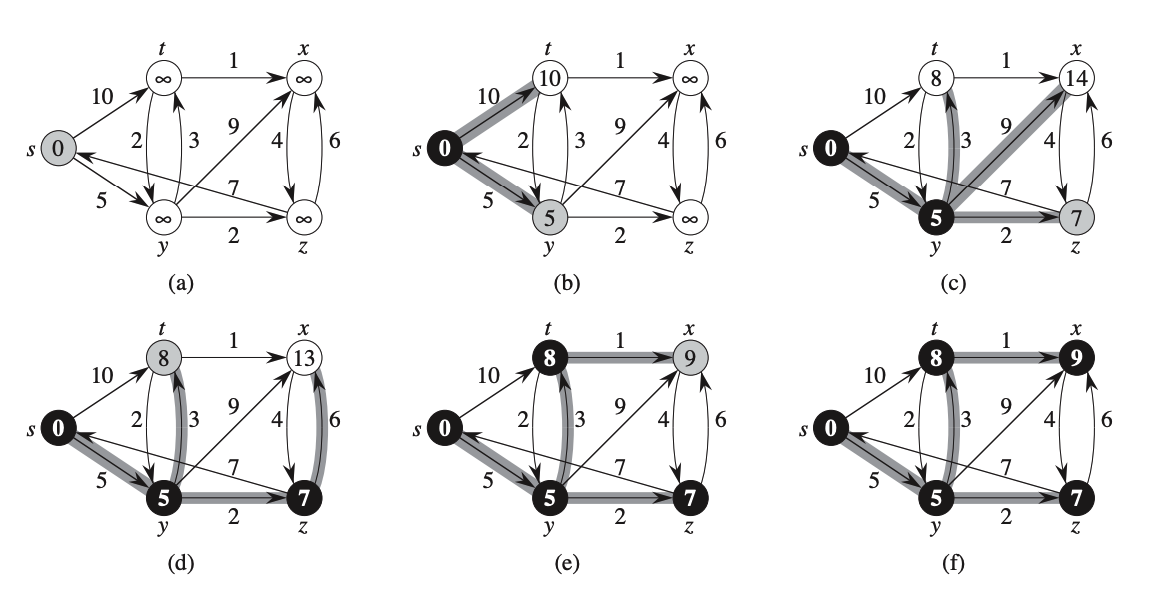
\includegraphics[width=\textwidth,height=\textheight,keepaspectratio]{alg-dijkstra.png}
    \caption{A execução do algoritmo de Dijkstra. O $s$ de origem é o vértice mais à esquerda. As estimativas de caminho mais curto aparecem dentro dos vértices e as bordas sombreadas indicam os valores predecessores. Os vértices pretos estão no conjunto $S$ e os vértices brancos estão na fila de prioridade mínima $Q = V - S$. (a) A situação imediatamente antes da primeira iteração do \emph{loop while} das linhas 5 – 9. O vértice sombreado tem o valor $d$ mínimo e é escolhido como vértice $u$ na linha 6. (b) - (f) A situação após cada iteração sucessiva do laço \emph{while}. O vértice sombreado em cada parte é escolhido como vértice $u$ na linha 6 da próxima iteração. Os valores $d$ e predecessores mostrados na parte (f) são os valores finais \cite{cormen2009}.}
    \label{sec3:alg-dijkstra}
\end{figure}

\begin{definition}
	O algoritmo de Dijkstra, executado em um grafo direcionado ponderado $G = (V, E)$ com função de peso não negativa $w$ e fonte $s$, termina com $u.d = \delta(s, u)$ para todos os vértices $u \in V$.
\end{definition}

%----------------------------------------------------------------------------------------
%	Árvore de caminhos mínimos
%----------------------------------------------------------------------------------------
\section{Árvore de caminhos mínimos}
Uma árvore de caminhos mínimos de um vértice $u$ é uma árvore geradora $T_u$ de $G$, de modo que o caminho de $u$ para todos os outros vértices de $T_u$ é um caminho mínimo em $G$. Tomaremos a árvore de caminho mínimos para um vértice $u$ como sendo $T_u$. Um caminho mínimo que começa na raiz de uma árvore Dijsktra é chamado de ramo de $G$. Mais formalmente, dado $T_u$, para cada $v \neq u$, o caminho mínimo de $u$ a $v$ é um ramo, denotado por $\mathcal{B}_u(v)$. Além disso, cada subcaminho de $\mathcal{B}_u(v) = p_{uv}$ é também um caminho mínimo em $G$, e denotamos esse conjunto de subcaminhos (incluindo $p_{uv}$) como $S(p_{uv})$ ou $S(\mathcal{B}_u(v))$ (ambas as notações são usadas indistintamente, por conveniência). Uma vez que $G$ não é direcionado, o mesmo se aplica a caminhos em ordem reversa, ou seja, cada subcaminho de $p_{vu}$ em $T_u$ também é um caminho mínimo. Com isto, assumimos $S(p_{vu})$ como sendo este conjunto de caminhos mínimos \cite{alane2021}.

%----------------------------------------------------------------------------------------
%	Caminhos mínimos entre todos os pares de vértices (APSP)
%----------------------------------------------------------------------------------------
\section{Caminhos mínimos entre todos os pares de vértices (APSP)}
O APSP, do inglês, {\it all pairs shortest paths} é o problema de calcular o comprimento mínimo entre cada par de vértices em um grafo ponderado. O problema APSP é muito bem estudado e tem havido resultados recentes para uma variedade de suposições para o grafo de entrada (direcionado, não direcionado, ponderado, não ponderado, etc.) \cite{alane2021} \cite{williams2014} \cite{pettie2002}.

%----------------------------------------------------------------------------------------
%	Complexidade de tempo
%----------------------------------------------------------------------------------------
\section{Complexidade de tempo}
O tempo de execução no pior caso para o algoritmo de Dijkstra em um grafo com $n$ nós e $m$ arestas é $\theta((m + n)log(n))$. Ele até encontra os caminhos mais curtos de um nó de origem $s$ para todos os outros nós no grafo. Isso é basicamente $O(n\log{}n)$ para seleção de nó e $O(m)$ para atualizações de distância. Embora $O(n\log{}n)$ seja a melhor complexidade possível para grafos densos, a complexidade pode ser melhorada significativamente para grafos esparsos. Com pequenas modificações, o algoritmo de Dijkstra pode ser usado como um algoritmo reverso que mantém árvores geradoras mínimas para o nó sorvedouro. Com outras modificações, ele pode ser estendido para se tornar bidirecional. O gargalo no algoritmo de Dijkstra, caso o grafo seja esparso, é a seleção de nós. No entanto, usando a implementação de Dial, isso pode ser melhorado significativamente para grafos esparsos \cite{len2021}.

É possível resolver o problema de encontrar os caminhos mínimos de todos os pares de vértices de um grafo, executando um algoritmo de caminhos mínimos de fonte única $|V|$ vezes, uma vez para cada vértice como fonte. Se todos os pesos das arestas forem não negativos, podemos usar o algoritmo de Dijkstra. Existem variações deste algoritmo, otimizando a complexidade de tempo, o mais famoso deles, o algoritmo de Floyd-Warshall, cuja complexidade de tempo é $\theta(n^3)$ e depende apenas de $n$.

%----------------------------------------------------------------------------------------
%	Centralidade de intermediação (betweenness centrality)
%----------------------------------------------------------------------------------------
\section{Centralidade de intermediação (\emph{betweenness centrality})}
A centralidade de intermediação é uma maneira de detectar a quantidade de influência que um nó tem sobre o fluxo de informações em um grafo. Em outras palavras, usa-se para localizar os nós que servem como "ponte" de uma parte de um grafo para outra ou que inferem possuir maior "importância".

Com o cálculo de todos os pares de caminhos mínimos em um grafo, os nós recebem uma pontuação, esta se refere a um montante de "importância" do nó em relação ao número de caminhos mínimos que passam pelo nó. Resumindo, os nós que mais frequentemente estiverem presentes nos caminhos mínimos de um grafo terão pontuações de centralidade de intermediação mais altas.

A Figura~\ref{sec3:graph-betweenness} apresenta um grafo não direcionado colorido com base na centralidade da intermediação de cada vértice do menor (vermelho) ao maior (azul).

\begin{figure}[!htb]
    \centering
    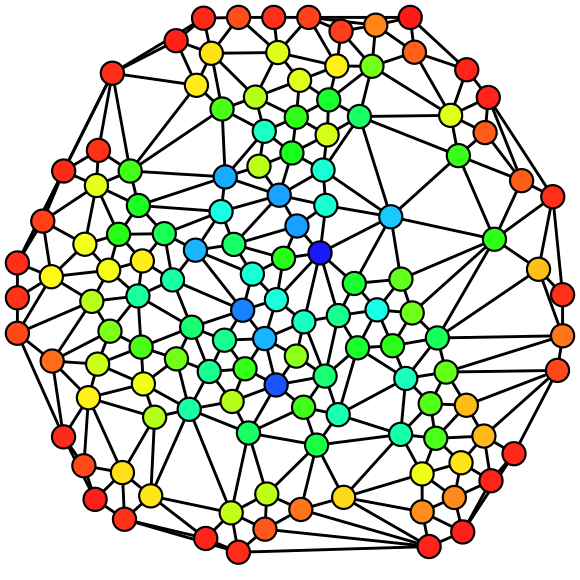
\includegraphics[scale=0.4]{graph-betweenness.png}
    \caption{Grafo não direcionado com as centralidades de intermediação dos vértices.}
    \label{sec3:graph-betweenness}
\end{figure}

Nesta mesma linha, podemos avaliar a "importância" de arestas ou, de forma mais relevante, dos caminhos mínimos, atribuindo-lhes pontuações toda vez que estes estão presentes como sub caminhos mínimos em outros caminhos mínimos. Isto desperta a importância e motiva ao estudo de, assim como na centralidade de intermediação em vértices, a centralidade de caminhos mínimos que será discutido na próxima seção.

%----------------------------------------------------------------------------------------
%	Centralidade de caminhos mínimos
%----------------------------------------------------------------------------------------
\section{Centralidade de caminhos mínimos}
A seguir apresento a definição da centralidade de caminhos mínimos de um grafo.

\begin{definition}
    (Centralidade de caminhos mínimos) Dado um grafo não direcionado ponderado $G = (V, E)$ com $n = |V|$, um par $(u, v) \in V^2$ e a árvore Dijkstra $T_a$ para cada $a \in V$, sejam $p_{ab} = (a,...,b)$ e $p_{uv} = (u,...,v)$ os caminhos mínimos de $a$ para $b$ e $u$ para $v$, respectivamente, tais que $p_{ab}, p_{uv} \in S(G)$. A centralidade do caminho mínimo de um par $(u, v) \in V^2$ é definida como
    \begin{align*}
        c(u, v) &= \frac{t_{uv}}{n(n - 1)}
    \end{align*}
    onde
    \begin{align*}
        t_{uv} &= \sum_{(a,b) \in V^2 : a \neq b} \mathbb{1}_{\tau_{uv}(\mathcal{B}_a(b))}
    \end{align*}
\end{definition}

A função $\mathbb{1}_{\tau_{uv}(\mathcal{B}_a(b))}$ retorna 1 se houver algum caminho mínimo de $u$ a $v$ como subcaminho do ramo $\mathcal{B}_a(b) \in S (T_a)$ (e 0 caso contrário). Intuitivamente falando, um par $(u, v)$ tem alta centralidade de caminho mínimo se o caminho mínimo canônico $p_{uv} \in S(T_u)$ (e $S(T_v)$) é um subcaminho de um grande número de caminhos canônicos mínimos em $S(G)$.

Considere o grafo da Figura~\ref{sec3:grafo-simples-5-nos}, o percurso mais curto do vértice $v_1$ para o vértice $v_3$ é o caminho mínimo $(v_1, v_3)$. Calculando-se todos os possíveis pares de caminhos mínimos deste grafo, chegaremos a conclusão de que o caminho mínimo $(v_1, v_3)$ terá maior centralidade que o caminho mínimo $(v_1, v_5, v_4)$ (percurso mais curto do vértice $v_1$ para o $v_4$) por exemplo, isto porque as vezes em que o caminho mínimo $(v_1, v_3)$ está presente como subcaminho mínimo é maior que as vezes em que o caminho mínimo $(v_1, v_5, v_4)$ está presente em outros.

\begin{figure}[!htb]
    \centering
	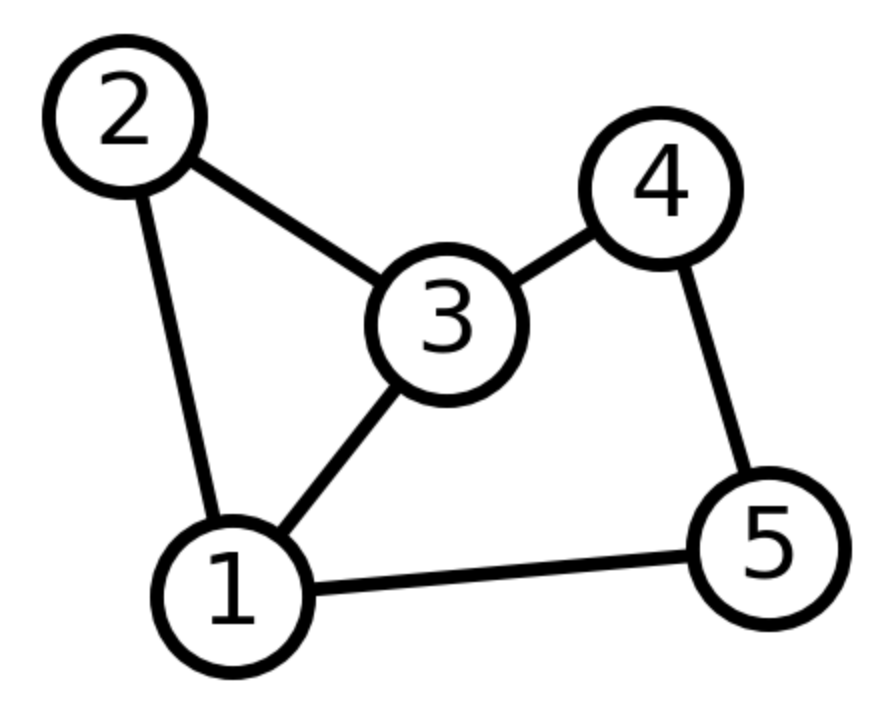
\includegraphics[scale=0.4]{grafo-simples-5-nos.png}
    \caption{Grafo simples com 5 nós.}
    \label{sec3:grafo-simples-5-nos}
\end{figure}

Assim como ocorre com o problema da centralidade de intermediação, a melhor maneira conhecida de se computar a centralidade de caminhos mínimos também é utilizando algoritmos que resolvem o APSP.

%----------------------------------------------------------------------------------------
%	Redundância de caminhos mínimos
%----------------------------------------------------------------------------------------
\section{Redundância de caminhos mínimos}
Adicionalmente, ainda considerando o grafo da Figura~\ref{sec3:grafo-simples-5-nos}, do vértice $v_1$ ao vértice $v_4$, um algoritmo de busca por caminhos mínimos pode retornar o percurso mais curto como sendo $<v_1, v_3, v_4>$ ou $<v_1, v_5, v_4>$, porém nos importa apenas uma destas saídas e usaremos a que o algoritmo em questão encontrar. Para a busca de caminhos mínimos, usaremos o algoritmo de Dijkstra e assumiremos seu retorno como verdade. Esta informação é importante e curiosa, pois dependendo de como o algoritmo se comporta/ trata os dados, o resultado do conjunto de caminhos mínimos podem diferir e, consequentemente, os valores de centralidade dos caminhos mínimos nos grafos que possuam mais de uma opção de percurso mais curso de entre um par de vértices. Este aspecto de aleatorização dos rótulos de um grafo é, inclusive, uma linha de pesquisa neste mesmo escopo, mas algumas bibliografias já indicam que, em grafos muito esparsos, a aleatorização dos rótulos não resulta em diferenças significativas nos valores de centralidade dos caminhos mínimos \cite{alane2021}.